\chapter{Evaluation}
\label{chap:evaluation}

Questions the evaluation needs to answer:

\begin{enumerate}
\item Show the implementations do not impose undue performance overheads on standard microkernel
operations.
\item Show that criticality mode switch is bounded by high criticality threads.
\item Show the cost of various timeout exception recovery mechanisms.
\item Show that temporal isolation is achieved.
\item Show that deadlines can be met during and after a mode switch.
\item Show the API is pracitcal and consistent with existing frameworks for critical software.
\end{enumerate}

\section{Hardware}

% describe benchmark setup, details of each hardware platform
In addition to several load generators running Linux on experiments are conducted on:

\begin{description}
    \item[ARM:] Quad-core 1\,GHz ARM Cortex~A9 system-on-chip on a Freescale i.MX6 SABRE Lite development board,
    \item[x64:] Quad-core 3.1\,GHz 64-bit Haswell i7-4770 machine.
\end{description}

\section{Overheads}

We first present a suite of microbenchmarks to evaluate any performane overheads against baseline seL4.
For each benchmark we ensure \gls{FPU} context switching is off by performing the required number of
without activating it such that the kernel will cease switching the FPU context. We present
overheads on IPC operations, signalling and irqs, and finally scheduling. 

% TODO measure the cost to reprogram the timer, read the timer

\subsection{IPC performance}

\Gls{IPC} performance is a critical measure of the practicality and efficiency of a
microkernel~\citep{Liedtke_95}. We benchmark our \gls{IPC} operations against base system, \selfour,
which has established performant \gls{IPC} fastpath~\citep{Elphinstone_Heiser_13}. 

\begin{table}[ht]\centering
\begin{tabular}{|c|l| r@{~}l | r@{~}l |r@{~}r|}\hline
\textbf{Arch}           & \multicolumn{1}{c|}{\textbf{Operation}}
                                & \multicolumn{2}{c|}{\textbf{Base}}
                                & \multicolumn{2}{c|}{\textbf{MCS}}
                                & \multicolumn{2}{c|}{\textbf{Overhead}} \\ \hline
\multirow{7}{*}{ARM}
\input{data/generated/sabre-ipc-micro.inc}
\hline
\multirow{7}{*}{x64}
\input{data/generated/haswell-ipc-micro.inc}
\hline
\end{tabular}
\caption{Microbenchmarks of seL4 IPC costs on seL4 baseline vs. MCS kernels. Standard deviations
shown in brackets.}
\label{t:micro}
\end{table}

To evaluate IPC performance we set up a client (the caller) and server (the callee) in different
address spaces. We take
timestamps on either side of the IPC operation being benchmarked and record the difference. This is
done 16 times for each result value to prime the cache, then record the next value. Results
presented are for performing this a total of 16 times. Additionally, we measure the overhead of
system calls stubs in the same way and subtract this from the measurement, to obtain only the kernel
cost of the operation\footnote{The IPC bencharmarks already existed for seL4, but were modified to
support the \gls{MCS} abi during the work for this thesis}. The message sent is zero length, so not
neither the caller or callee's \gls{IPC} buffer acessed.
This is done for both directions of IPC, as described in \Cref{sec:seL4-api}. 

We evaluate the \gls{IPC} fastpath and various slowpaths: slowpath between passive threads and
active threads, and the fault path, where the caller is the faulting process and the callee is the
fault handler.

Fastpath results for \call and \replyrecv increase by a few percent on each platform,
resulting from extra checks on the fastpath to
accommodate scheduling contexts, an extra capability lookup for the Resume object, touching two
separate new objects (\gls{SCO} and Resume object) and enforcing priorities
on IPC delivery (baseline does \gls{FIFO}).

Slowpath results show the greater cost of the model. 

\autoref{t:micro} shows the cost of the (performance-wise) most
important kernel operations of our present implementation (MCS), compared to
the baseline seL4 kernel (base). \code{call()} is the client-style
invocation, which sends a message to an IPC endpoint (port),
 blocking until it receives until receiving a reply.
We measure IRQ latency using two thread, one spinning in a loop
updating a volatile cycle counter, the other, higher priority thread
waiting for an interrupt. On delivery, the handler thread determines the
IRQ latency by subtracting the
looped timestamp from the current time. The overhead is higher here as we must switch scheduling
contexts, which requires reprogramming the timer.

\subsection{Signalling and IRQS}

\begin{table}[h]\centering
\begin{tabular}{|c|l| r@{~}l | r@{~}l |r@{~}r|}\hline
\textbf{Arch}           & \multicolumn{1}{c|}{\textbf{Operation}}
                                & \multicolumn{2}{c|}{\textbf{Base}}
                                & \multicolumn{2}{c|}{\textbf{MCS}}
                                & \multicolumn{2}{c|}{\textbf{Overhead}} \\ \hline
\multirow{3}{*}{ARM}
\input{data/generated/sabre-irq-micro.inc}
\hline
\multirow{3}{*}{x64}
\input{data/generated/haswell-irq-micro.inc}
\hline
\end{tabular}
\caption{Microbenchmarks of seL4 signal and IRQ latency on seL4 baseline vs. MCS kernels. Standard deviations
shown in brackets.}
\label{t:micro-irq}
\end{table}

The \code{signal()} operation signals a Notification object (semaphore). This microbenchmark evaluates the cost of signalling a lower priority thread -- no scheduling context switch occurs, but the kernel
reads the timestamp timestamp is updated unnecessarily and rolled back as shown in \autoref{figure:tickless}.


\subsection{Scheduling}

\begin{table}[ht]\centering
\begin{tabular}{|c|l| r@{~}l | r@{~}l |r@{~}r|}\hline
\textbf{Arch}           & \multicolumn{1}{c|}{\textbf{Operation}}
                                & \multicolumn{2}{c|}{\textbf{Base}}
                                & \multicolumn{2}{c|}{\textbf{MCS}}
                                & \multicolumn{2}{c|}{\textbf{Overhead}} \\ \hline
\multirow{4}{*}{ARM}
\input{data/generated/sabre-schedule-micro.inc}
\hline
\multirow{4}{*}{x64}
\input{data/generated/haswell-schedule-micro.inc}
\hline
\end{tabular}
\caption{Microbenchmarks of seL4 IPC scheduling costs.}
\label{t:micro-schedule}
\end{table}

The \code{schedule} benchmark measures the cost of a signal to a higher priority thread, which forces a reschedule.
Scheduling cost increases noticeably due to the need for first reading
and then reprogramming the timer for budget enforcement. Furthermore,
the sporadic replenishment logic is far more complicated than the
previous tick-based logic, and there is some extra code for
dealing with scheduling contexts. Note that seL4 IPC,
particularly scheduler-context donation (and its predecessor, the
undisciplined timeslice donation), is designed to minimise the need for
invoking the scheduler, therefore this increase is unlikely to have
a noticeable effect in practice. In fact, the \(O(1)\) scheduler is a
recent addition to seL4: scheduling used to be far more expensive.

The SMP benchmark is an IPC throughput benchmark, which sets up pairs of IPC ping-pong
(pong is passive on MCS) threads on each of 2 cores, and for a delay between 0 and 500 cycles.
We show a slight degredation in IPC throughput on x86, due to the increase in fastpath.

All in all, our overheads are reasonable given the speed of the baseline kernel and the extend of
the provided functionality.

\subsection{SMP}

\begin{table}[ht]\centering
\begin{tabular}{|c|l| r@{~}l | r@{~}l |r@{~}r|}\hline
\textbf{Arch}           & \multicolumn{1}{c|}{\textbf{Operation}}
                                & \multicolumn{2}{c|}{\textbf{Base}}
                                & \multicolumn{2}{c|}{\textbf{MCS}}
                                & \multicolumn{2}{c|}{\textbf{Overhead}} \\ \hline
%\multirow{5}{*}{ARM}
%\input{data/generated/sabre-ipc-micro.inc}
%\hline
%\multirow{6}{*}{x64}
%\input{data/generated/haswell-ipc-micro.inc}
& SMP xput & \multicolumn{2}{l|}{1,454,260} & \multicolumn{2}{l|}{1,389,198} & 65k & 4.6\% \\
\hline
\end{tabular}
\caption{SMP throughput}.
\label{t:micro-smp}
\end{table}

\subsection{Temporal Isolation}

% Show isolation between processes using different scheduling contexts
\paragraph{Process isolation} We demonstrate our isolation properties
in a single-core setup consisting of a Linux VM,
running at high priority with a
constrained budget and a UDP echo server running at a lower priority,
representing a lower-rate \textsc{high} thread, illustrated in \autoref{f:ipbench-arch}. We
measure the average  and maximum UDP latency reported by the
ipbench~\citep{Wienand_Macpherson_04} latency test.

Specifically, the Linux VM interacts with timer (PIT) and serial device drivers implemented as
passive servers outside the VM; all three components are at a high priority. In the Linux server we
run a program (\code{yes > /dev/null}) which consumes all available
CPU bandwidth.  The UDP echo server, completely isolated from the Linux instance, but sharing the serial driver,
runs at a low priority.

\begin{figure}[ht]
    \centering
    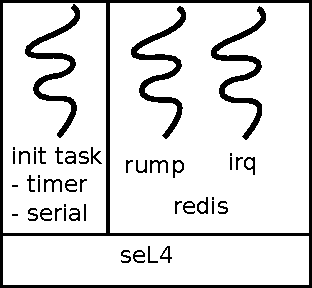
\includegraphics{redis-arch}
    \caption{Architecture of the networking benchmarks. Dotted lines
    \label{f:redis-arch}
    are passive-server threads.}
\end{figure}


\begin{figure}[ht]
    \centering
    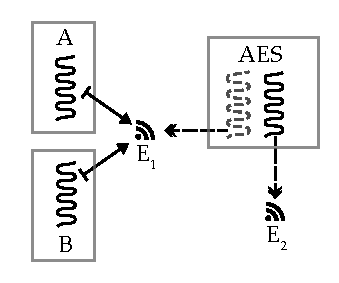
\includegraphics{ipbench-arch}
    \caption{Architecture of the ipbench benchmark. Dotted lines
    are passive-server threads.}
    \label{f:ipbench-arch}
\end{figure}


Two client machines run ipbench daemons to send packets to the UDP-echo server on the target machine
(Haswell platform). The control machine, one of the load generators, runs ipbench with a \gls{UDP} socket at 10\,Mbps over a 1\,Gb/s Ethernet connection with 100-byte packets. The Linux VM has a 10\,ms period and we vary the
budget between 1\,ms and 9\,ms.
%We represent the zero-budget case by an unconstrained Linux that is not running any user code.
Any time not consumed by Linux is available to UDP echo for processing
10,000 packets per second, or 100 packets in the time left over from
each of Linux's 10\,ms period.

\begin{figure}[t]
  \centering
  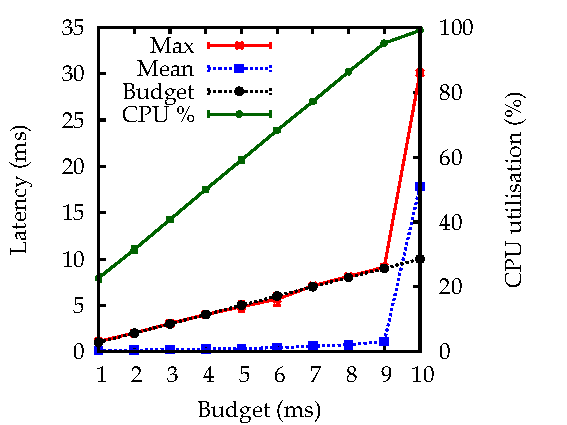
\includegraphics[width=0.9\columnwidth]{ipbench}
  \caption{Average and maximum latency of UDP packets with a
    CPU hog running a high priority with a 10\,ms budget.}
  \label{f:ipbench}
\end{figure}

\autoref{f:ipbench} shows the average and maximum UDP latencies for
ten runs at each budget setting. We can see that the maximum latencies
follow exactly the budget of the Linux server (black line) up to 9\,ms. Only
when Linux has a full budget (10\,ms), and thus able to monopolise the
processor, does the UDP server miss its deadlines, resulting in a
latency blowout.  This result shows that our sporadic server implementation is effective in bounding interference of a high-priority process.

\paragraph{Network benchmark} We evaluate the overhead of our implementation and
again demonstrate temporal isolation by running the Yahoo! Cloud Serving Benchmark
(YCSB)~\citep{Cooper_STRS_10}.
 We run it against a server using the Redis
 key-value store~\citep{redis:url} with NetBSD~\citep{NetBSD:url} drivers at user-level provided
 by a single-core Rump library OS~\citep{Kantee_Cormack_14} on x86.

The system consists of Redis/Rump running on three active seL4 threads: two for servicing interrupts
(network, timer) and one for Rump, as shown in \autoref{f:redis-arch}.
Interrupt threads run at the highest priority, followed by Redis and
a low-priority idle thread (not shown) for measuring CPU utilisation;
this setup forces frequent invocations of the scheduler and interrupt
path. \autoref{t:redis} shows the achieved throughput of Redis+Rump
running  bare-metal (BMK), and Redis on the seL4 baseline and as well as the MCS
branch, plus Linux and NetBSD for comparison.

% TODO update
The utilisation figures show that the system is fully loaded, except
in the Linux case, where there is a small amount of idle time. The
cost per operation (utilisation over throughput) is best on Linux, a
result of its highly optimised drivers and network stack. Our
bare-metal and seL4-based setups use Rump's NetBSD drivers, and
actually achieve slightly better performance than NetBSD. This
indicates that our MCS support comes with low overhead.


\begin{table}[t]\centering
      \begin{tabular}{|c|c|c|c|c|}
        \hline
        \textbf{System (IRQ)}  & \textbf{Tput} & \textbf{Utilis.} &  \textbf{Latency} \\
                               & (k ops/s)     &  (\%)            &   (ms)            \\
        \hline
      \input{data/ycsb-redis.inc}
    \end{tabular}
    \caption{Throughput (k\,ops/s) achieved by Redis using the YCSB
      workload A ith 2 clients.  Latis average Read and Update,
      standard deviations in brackets.}
    \label{t:redis}
\end{table}

We next run Redis with a high-priority CPU-hog thread competing for CPU time. All threads have a
5\,ms period. We use the budget of the hog to control the amount of time left over
for the server configuration. \autoref{f:redis} shows the throughput
achieved by the YCSB-A workload as a function of the available CPU
bandwith (i.e \ the complement of the bandwidth granted to the hog
thread). Each data point is the average of three benchmark runs.

\begin{figure}[t]
  \centering
  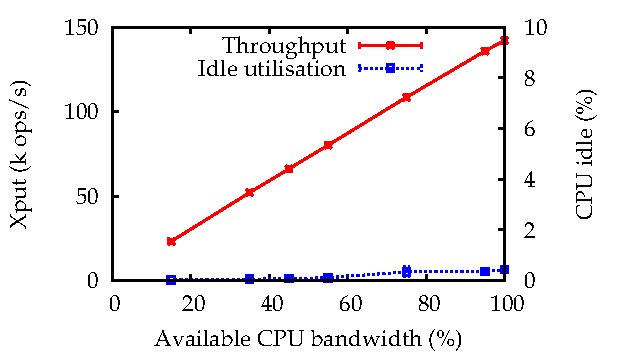
\includegraphics{redis}
  \caption{Throughput of Redis YCSB workload A and idle time vs available bandwidth.}
  \label{f:redis}
\end{figure}

The graph shows that the server is CPU limited (as indicated by very low idle time)
and consequently throughput scales linearly with available CPU
bandwidth.

% Show isolation in a shared server
\paragraph{Server isolation} As an example of a shared server running out of budget, we implement
the scenario of a passive server (see \autoref{f:passive}) with two
clients, A and B. The server is providing an encryption service using AES-256
with a block size of 16~bytes. The server alternates between two
buffers, of which one always contains consistent state, the other is
dirty during processing. Both clients request 4\,MiB of data to be encrypted, and
have budget insufficient to complete the request (budgets of 1\,ms and
5\,ms with a 10\,ms period).

\begin{table}[t]\centering
\begin{tabular}{|c|l|l|r|r|r|r|}\hline
\textbf{Arch} & \textbf{Op.} & \textbf{Cache} & \textbf{Min} &
                          \textbf{Max} & \textbf{Mean} &
                          \multicolumn{1}{c|}{\boldmath \(\sigma\)} \\\hline
\multirow{8}{*}{ARM} \input{data/generated/sabre-aes.inc} \hline
\multirow{8}{*}{x64} \input{data/generated/haswell-aes.inc} \hline
\end{tabular}
\caption{Cost of timeout handler operations in \(\mu\)s, as measured
  by timeout exception handler. \(\sigma\) is the standard deviation.}
\label{t:rollback}
\end{table}

\begin{figure*}[t]
  \centering
  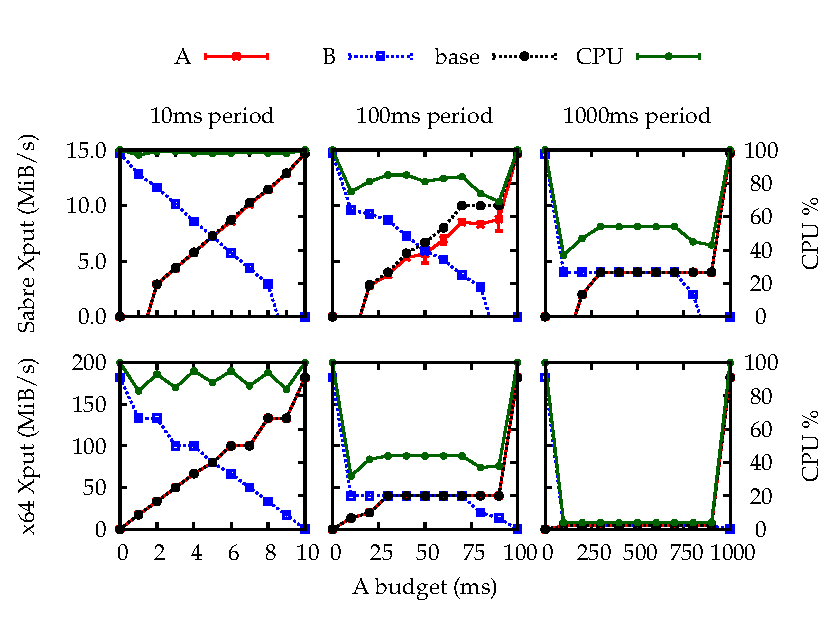
\includegraphics[width=\textwidth]{aes-shared}
  \caption{Throughput for clients A and B of a passive AES server processing 10 requests of 4\,MiB of data with
      limited budgets on the x64 (top row) and ARM (bottom row) platforms. The two clients' budgets
      add up to the period, which is varied between graphs (10, 100, 1000\,ms). Clients sleep when
      they process each 4\,MiB, until the next period, except when their budgets are full. Each data point is the average of 10 runs, error bars show the standard deviation.}
  \label{f:aes}
\end{figure*}

When the server runs out of budget, its timeout exception handler gets
invoked. We implement 4 different strategies for handling timeout exceptions,
and measure the latency of timeout handling, from the time the handler wakes up
until it replies to the server.

\emph{Rollback (RB)} rolls the server back to the last consistent state
recorded and replies to the client on behalf of the server with the amount of data
encrypted so far. The faulting client can then continue its request once its budget is replenished.
We measure rollback time, from the time the exception handler is
invoked, until the server is ready for the next request. Given the
small amount of rollback state, this measures the baseline
overhead. For schedulability analysis, the actual cost of the rollback would
have to be added.

\emph{Emergency (Emg.)} gives the server a one-off emergency budget to finish
the client request, after which the exception handler
resets the server to being passive. The benchmark measures the
pure handling overhead, the actual request completion time must again be added.

\emph{Extend (Ext.)} simply increases the client's budget on each timeout while \emph{Kill} destroys the client.

We run the benchmarks with hot caches (primed by some warmup
iterations)  as well as cold (flushed) caches.

\autoref{t:rollback} shows the results. The maximum
cold-cache cost, which is relevant for schedulability analysis,
differs by a factor of 3--4 between the different recovery scenarios,
indicating that all are about equally feasible.
Approaches that restart the server (RB, Kill) are the most expensive
as they must restore the server state from a
checkpoint and follow the passive server initialisation protocol
(recall \autoref{s:passive}). This requires
5 system calls in each case for killing or replying to the client and RPC-ing to the server.

We next demonstrate temporal isolation in the server by using the RB
technique and measuring the time taken to encrypt 10 requests of 4\,MiB of
data. \autoref{f:aes} shows the result with both clients having the same
period, which we vary between 10\,eft graphs) and 1\,s
(right). In each graph  we vary the clients' budget between 0 and the
period. The extreme ends are special, as one of the clients has a full
budget and keeps invoking the server without ever getting rolled back,
thus monopolising the processor. In all other cases, each client
processes at most 4\,MiB of data per period, and either succeeds (if
the budget is sufficient) or is rolled back after processing less than 4\,MiB.

The results that in the CPU-limited cases (left graphs)
we have the expected near perfect proportionality between throughput and
budget (with slight wiggles due to the rollbacks), showing isolation between clients. In the cases where there is headspace (centre of the right
graphs), both clients achieve their desired throughput.

\subsection{Criticality}

We evaluate our kernel mechanism for changing criticaliwith two benchmarks: A
microbenchmark measuring the cost of a mode switch, and another showing deadline misses of threads sets over several mode changes.

\begin{figure}[t]
  \centering
  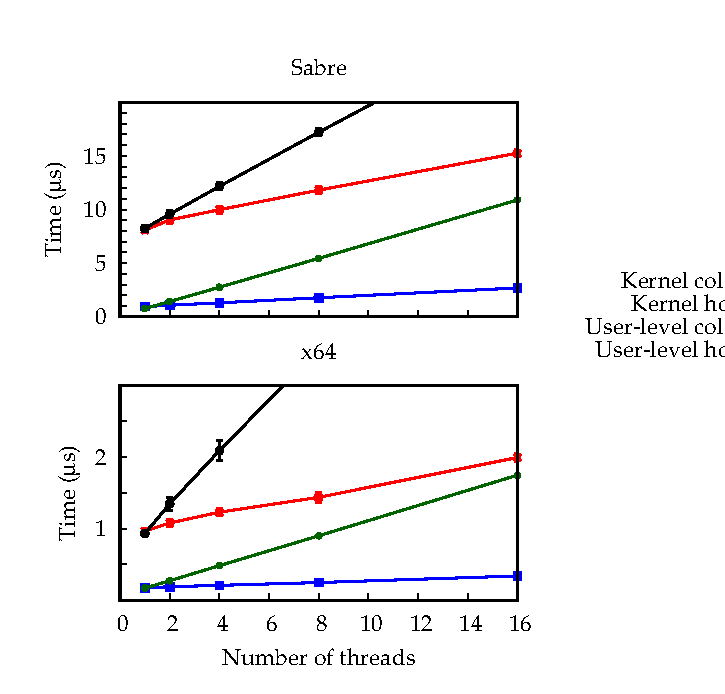
\includegraphics[width=\linewidth]{mode-switch-all}
  \caption{Cost of switching the priority of $n$ threads, as well as changing from \crit{low} to
  \crit{high} criticality level while increasing the number of \crit{high} and \crit{low} threads,
  on Sabre and Haswell. Each data point is the average of 100 runs, with very small standard
  deviations.}
  \label{f:mode-switch}
\end{figure}

To evaluate the cost of changing the system criticality level, we
configure the kernel with 128 priorities and 2 criticality levels
(0--1). We then  run 3 experiments as follows:
\iffalse                        % OLD
\begin{itemize}
\item \textbf{UL:} measures the time to change the priority of $n$ threads from user-level;
\item \textbf{HI:} measures the time for raising the system criticality level from 0 to 1 with one \crit{low} thread and $n$
    \crit{high} threads, i.e.\ threads whose priority must be boosted upon criticality switch,
\item \textbf{LO:} measures the time for raising the system criticality level from 0 to 1 with one \crit{high} thread and
 } threads, whose priority does not need to be boosted.
\end{itemize}
\else                           % PREFERRED
\begin{description}
\item[UL:] measures the time to change the priority of $n$ threads from user-level;
\item[HI:] measures the time for raising the system criticality level from 0 to 1 with one \crit{low} thread and $n$
    \crit{high} threads, i.e.\ the priority of $n$ threads must be boosted;
\item[LO:] measures the time for raising the system criticality level from 0 to 1 with one \crit{high} thread and
    $n$ \crit{low} threads, i.e.\ only one thread must be boosted.
\end{description}
\fi

\Cref{f:mode-switch} shows the results, where each data point is the result of 100 measurements.
We show results with a primed cache (hot) and flushed cache (cold).
As the graph shows, switching is linear in the number of \crit{high} threads being boosted. Varying the number
of \crit{low} threads has no impact on the execution time of a mode switch.
This is important, as the schedulability analysis for critical threads
must not depend on less-critical threads, and should not make
assumptions how many threads less-critical software creates.

In absolute terms, the results show that a mode switch is fairly fast,
remaining under 2\,$\mu$s on x64 and about 12\,\(\mu\)s on ARM for switching 8 threads
with a cold cache. Most systems will not have more than a few high
criticality threads, and deadlines for critical control loops in
cyber-physical systems tend to be in the tens of milliseconds, meaning
that budgeting a few microseconds for an emergency mode switch is eminently
feasible.

Additionally, the results show that changing the priority at user-level, rather than using the
criticality boost, is also linear in the number of threads to be boosted, but  is significantly slower than using the kernel mechanism (i.e.\ mode switch).
The higher cost from user-level operation results from  multiple switches between kernel and user mode, and the repeated thread-capability look-ups.

% TODO mode switch benchmark
For our second mode-switch benchmark, we ported 3 processor intensive benchmarks from the
MiBench~\citep{Guthaus_REAMB_01} to act as workloads. Each benchmark runs in its own Rump process
with an in-memory fem, and shares a timer and serial server.

We altered the benchmarks to run periodically in multiple stages. To obtain
execution times long enough, some of the benchmarks iterate a fixed number of times per
stage. Each benchmark process executes its workload and then waits for the next period to start.
Deadlines are implicit: if a periodic job finishes before the start of the next period it is
considered successful, otherwise the deadline is missed.

\Cref{t:modeswitch} lists the benchmarks with periods and criticalities.
\textit{susan}, the most critical, has three stages: edge detection, smoothing, and corners. The
next critical task, \textit{jpeg}, has two stages: encode, and decode. The least
critical task, \textit{mad} has only one stage. We run the benchmark
for 20\,s for each of the stages (repeating the last phase where
threads have no new phase), and
increment the system criticality level at stage transition. The parameters are arranged such that
rate-monotonic priorities are inverse to the criticalities.

Results are shown in \autoref{t:modeswitch}. For stage one, the entire workload is schedulable and
there are no deadline misses. For stage two, the workload is not
schedulable, and the criticality switch boosts the priorities of
\textit{susan} and \textit{jpeg}, such that they meet
their deadlines, but
\textit{mad} does not. In the final stage, only the most critical task
meets all deadlines.
This shows that our mechanisms operate as intended.


\begin{table}[h]\centering
    \begin{tabular}{|l|c|c|c|c|}\hline
        \multicolumn{5}{|l|}{\textit{susan}, image recognition, \(L\): 2 \(T\): 180}\\\hline
        \textbf{\(L_S\)} & \textit{C} & \textit{U} & \textit{j} & \textit{m} \\\hline
                     0 & 25 & 0.14 & 111 & 0 \\\hline
                     1 & 51 & 0.15 & 111 & 0 \\\hline
                     2 & 127 & 0.54 & 111 & 0 \\\hline
        \multicolumn{5}{|l|}{\textit{jpeg}, encode/decode, \(L\): 1 \(T\): 100}\\\hline
        \textbf{\(L_S\)} & \textit{C} & \textit{U} & \textit{j} & \textit{m} \\\hline
                     0 & 15 & 0.15 & 200 & 0 \\\hline
                1 & 41 & 0.41 & 200 & 0 \\\hline
                     2 & 41 & 0.41 & 148 & 88 \\\hline
        \multicolumn{5}{|l|}{\textit{mad}, mp3 playing, \(L\): 0 \(T\): 112}\\\hline
        \textbf{\(L_S\)} & \textit{C} & \textit{U} & \textit{j} & \textit{m} \\\hline
                     0 & 28 & 0.25 & 179 & 0 \\\hline
                     1 & 28 & 0.25 & 178 & 46\\\hline
                     2 & 28 & 0.25 & 7 & 7 \\\hline
    \end{tabular}
    \caption{Results of mode switch benchmark for each
        stage, where the  criticality \(L_S\) is raised each stage. \(T\) =
        period, \textit{C} = worst observed execution time (ms),
      \textit{U} = allowed utilisation (budget/period),
    \textit{m} = deadline misses, \textit{j} = jobs completed. We recorded 52, 91 and 100\% CPU
utilisation for each stage respectively.}
    \label{t:modeswitch}
\end{table}


\subsection{Practicality}

\subsubsection{User-level scheduling}\label{s:edf-impl}

Fundamental to the microkernel philosophy is keeping policy out of the
kernel as much as possible, and instead providing general mechanisms
that allow the implementation of arbitrary policies
\citep{Heiser_Elphinstone_16}.  As on the face of it, our
fixed-priority-based model seems to violate this principle,  we
demonstrate that the model is general enough to support the efficient
implementation of alternate policies at user level. Specifically, we
show that we can efficiently implement \gls{EDF}, the popular and  optimal dynamic-priority policy (see \autoref{s:theory}).

We implement the EDF scheduler as an active server with active
clients which run at an seL4 priority below the scheduler.
The scheduler waits on an endpoint on which it receives messages from
its clients or the timer.

Each client has a period which represents its relative deadline and a full reservation (i.e.\ equal to the period). Clients
either explicitly notify the scheduler of completion by an IPC
message, or else create a timeout exception on preemption, which is also received by the
scheduler. Either is an indication that the next thread should be scheduled.

We use the \emph{randfixedsum}~\citep{Emberson_SD_10} algorithm to
generate deadlines between 10 and 1000\,ms for a certain number of threads.
A set of threads runs until 100
scheduling decisions have been recorded. We repeat this 10 times,
resulting in 1,000 scheduler runs for each data point.

We measure the scheduler latency by recording the timestamp when each client thread, and an idle
thread, detects a
context switch and processing the difference in timestamp pairs offline. We run two schedulers:
\emph{pre}-empt where threads never yield and must incur a timeout exception, and \emph{coop}, where
threads use IPC to yield to the scheduler. The latter invokes the user level timer
driver more often as the release queue is nearly always full, which involves more kernel invocations
to acknowledge the IRQ, in addition to reprogramming the timer.

We compare our latencies to those of
LITMUS$^{RT}$~\citep{Calandrino_LBDA_07}, a widely-used real-time scheduling
framework embedded in Linux, where we use Feather-Trace~\citep{Brandenburg_Anderson_07} to gather data.
We use the C-EDF scheduler, which is a partitioned (per-core), clustered (per-node) EDF scheduler, on a single
core. We use the same parameters and thread sets, running each set for 10\,s. 
The measured overhead considers the in-kernel scheduler, context-switch and user-level code to return to
the user.

\autoref{f:edf} shows that our user-level EDF scheduler implementation is
competitive with t EDF from LITMUS$^{RT}$, and
that the cost of implementing scheduling policy at user level is of
the same order as the in-kernel default scheduler. In other words,
implementing different policies on top of the base scheduler is quite feasible.

\begin{figure}[t]
    \centering
    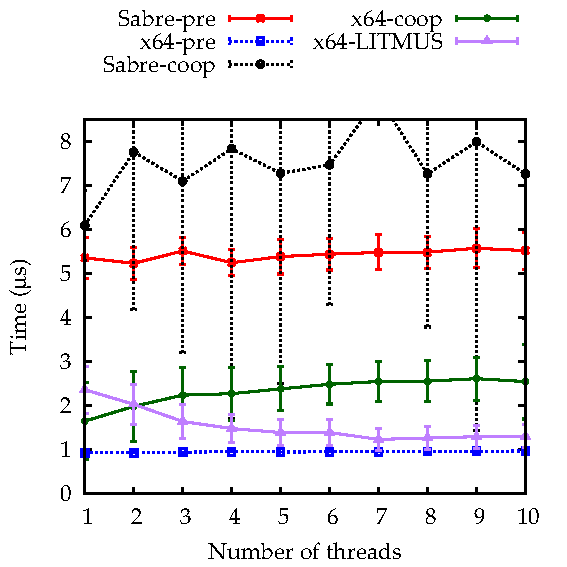
\includegraphics[width=0.9\linewidth]{edf}
    \caption{Execution time of seL4 user-mode EDF scheduler compared to
             kernel scheduler in x64 LITMUS$^{RT}$.}
    \label{f:edf}
\end{figure}


Our evaluation demonstrates our model has minimal overheads, achieves isolation,  provides a notion
of criticality orthogonal to priority, and allows for efficient user-level scheduling.
In total, we add 2,245 lines of SLOC~\citep{Wheeler_01} to the preprocessed kernel code for the sabre
(the verified platform), representing a 16\% increase.

